\documentclass[]{article}
\usepackage{geometry,tikz,lipsum,amsmath,amssymb,soul,xcolor,cancel,esint}

% Gradient Info

\tikzset {_t5mdhtxnp/.code = {\pgfsetadditionalshadetransform{ \pgftransformshift{\pgfpoint{0 bp } { 0 bp }  }  \pgftransformscale{1 }  }}}
\pgfdeclareradialshading{_y4oyjsov0}{\pgfpoint{0bp}{0bp}}{rgb(0bp)=(0.82,0.01,0.11);
	rgb(0bp)=(0.82,0.01,0.11);
	rgb(11.25bp)=(0.82,0.01,0.11);
	rgb(11.339285714285714bp)=(1,1,1);
	rgb(25bp)=(1,1,1);
	rgb(400bp)=(1,1,1)}
\tikzset{_7fj56osav/.code = {\pgfsetadditionalshadetransform{\pgftransformshift{\pgfpoint{0 bp } { 0 bp }  }  \pgftransformscale{1 } }}}
\pgfdeclareradialshading{_aykr5aomc} { \pgfpoint{0bp} {0bp}} {color(0bp)=(transparent!0);
	color(0bp)=(transparent!0);
	color(11.25bp)=(transparent!0);
	color(11.339285714285714bp)=(transparent!100);
	color(25bp)=(transparent!100);
	color(400bp)=(transparent!100)} 
\pgfdeclarefading{_bcb2u9fkc}{\tikz \fill[shading=_aykr5aomc,_7fj56osav] (0,0) rectangle (50bp,50bp); } 

% Gradient Info

\tikzset {_86h7qoix5/.code = {\pgfsetadditionalshadetransform{ \pgftransformshift{\pgfpoint{0 bp } { 0 bp }  }  \pgftransformscale{1 }  }}}
\pgfdeclareradialshading{_6rp8budzf}{\pgfpoint{0bp}{0bp}}{rgb(0bp)=(0.22,0.6,0.72);
	rgb(0bp)=(0.22,0.6,0.72);
	rgb(11.25bp)=(0.22,0.6,0.72);
	rgb(11.339285714285714bp)=(1,1,1);
	rgb(25bp)=(1,1,1);
	rgb(400bp)=(1,1,1)}
\tikzset{_vav0c5zdw/.code = {\pgfsetadditionalshadetransform{\pgftransformshift{\pgfpoint{0 bp } { 0 bp }  }  \pgftransformscale{1 } }}}
\pgfdeclareradialshading{_dekypsmmo} { \pgfpoint{0bp} {0bp}} {color(0bp)=(transparent!0);
	color(0bp)=(transparent!0);
	color(11.25bp)=(transparent!0);
	color(11.339285714285714bp)=(transparent!100);
	color(25bp)=(transparent!100);
	color(400bp)=(transparent!100)} 
\pgfdeclarefading{_okjtkvlfh}{\tikz \fill[shading=_dekypsmmo,_vav0c5zdw] (0,0) rectangle (50bp,50bp); } 
\tikzset{every picture/.style={line width=0.75pt}} %set default line width to 0.75pt

\numberwithin{equation}{section}

\NewDocumentCommand{\caja}{ m O{gray!40} O{gray!10} m }{
	\begin{figure}[h]
		\centering
		\begin{tikzpicture}
			\node[anchor=text, text width=\columnwidth-1.2cm, draw, rounded corners, line width=1pt, fill=#3, inner sep=5mm] (big) {\\#4};
			\node[draw, rounded corners, line width=.5pt, fill=#2, anchor=west, xshift=5mm] (small) at (big.north west) {#1};
		\end{tikzpicture}
	\end{figure}
}
\NewDocumentCommand{\indUpDown}{ O{\Lambda} O{\mu} O{\nu} }{
	{#1}^{#2}_{\ #3}
}
\NewDocumentCommand{\indDownUp}{ O{\Lambda} O{\mu} O{\nu} }{
	{#1}_{#2}^{\ #3}
}
\newcommand{\LambdaMuNu}{\indUpDown}
\newcommand{\0}{\textcolor{gray}{0}}
\newcommand{\rbf}{\mathbf{r}}
\newcommand{\ei}{\mathbf{e}_i}
\newcommand{\ej}{\mathbf{e}_j}
\newcommand{\lc}{\epsilon_{ijk}}

\newcommand{\la}{\nabla^2}
\newcommand{\rv}{\mathbf{r}}
\newcommand{\xv}{\mathbf{x}}
\newcommand{\yv}{\mathbf{y}}
\newcommand{\zv}{\mathbf{z}}
\newcommand{\vv}{\mathbf{v}}
\newcommand{\Vv}{\mathbf{V}}
\newcommand{\xhat}{\hat{\xv}}
\newcommand{\yhat}{\hat{\yv}}
\newcommand{\zhat}{\hat{\zv}}
\newcommand{\rhat}{\hat{\rv}}
\newcommand{\that}{\hat{\mathbf{\theta}}}
\newcommand{\phat}{\hat{\mathbf{\varphi}}}
\newcommand{\rhhat}{\hat{\mathbf{\rho}}}

\newcommand{\pd}[2]{\dfrac{\partial #1}{\partial #2}}
\newcommand{\td}[2]{\dfrac{d #1}{d #2}}

\newcommand{\wfrac}[3][3pt]{%
	\frac{\wfracterm{depth}{\dp}{#1}{#2}}{\wfracterm{height}{\ht}{#1}{#3}}%
}
\newcommand{\wfracterm}[4]{%
	\sbox0{$\displaystyle#4$}%
	\vrule width 0pt #1 \dimexpr #20+#3\relax
	\usebox{0}%
}

%opening
\title{Tarea 2 Mecánica Clásica Avanzada}
\author{Simon Fonseca}

\begin{document}
\maketitle
\section{Pregunta 1}
A homogeneous cone of mass \(m\), radius \(R\) and length \(\ell \gg R\) \underline{rolls} over the horizontal surface, as shown in the figure. The tip (vertex) of the cone does not move, but the cone can rotate freely around it.

\begin{figure}[h!]
	\centering
	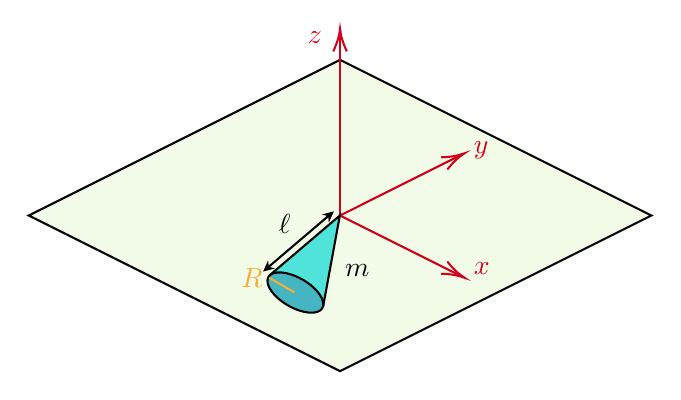
\begin{tikzpicture}[x=0.75pt,y=0.75pt,yscale=-1,xscale=1]
		%uncomment if require: \path (0,325); %set diagram left start at 0, and has height of 325
		
		%Straight Lines [id:da044362991789894] 
		\draw [fill={rgb, 255:red, 184; green, 233; blue, 134 }  ,fill opacity=0.2 ]   (165,20) -- (315,95) -- (165,170) -- (15,95) -- cycle ;
		%Straight Lines [id:da13048107665015474] 
		\draw [color={rgb, 255:red, 208; green, 2; blue, 27 }  ,draw opacity=1 ]   (165,95) -- (223.21,65.89) ;
		\draw [shift={(225,65)}, rotate = 153.43] [color={rgb, 255:red, 208; green, 2; blue, 27 }  ,draw opacity=1 ][line width=0.75]    (10.93,-3.29) .. controls (6.95,-1.4) and (3.31,-0.3) .. (0,0) .. controls (3.31,0.3) and (6.95,1.4) .. (10.93,3.29)   ;
		%Straight Lines [id:da34215627687454997] 
		\draw [color={rgb, 255:red, 208; green, 2; blue, 27 }  ,draw opacity=1 ]   (165,95) -- (223.21,124.11) ;
		\draw [shift={(225,125)}, rotate = 206.57] [color={rgb, 255:red, 208; green, 2; blue, 27 }  ,draw opacity=1 ][line width=0.75]    (10.93,-3.29) .. controls (6.95,-1.4) and (3.31,-0.3) .. (0,0) .. controls (3.31,0.3) and (6.95,1.4) .. (10.93,3.29)   ;
		%Straight Lines [id:da03370557352782089] 
		\draw [color={rgb, 255:red, 208; green, 2; blue, 27 }  ,draw opacity=1 ]   (165,95) -- (165,7) ;
		\draw [shift={(165,5)}, rotate = 90] [color={rgb, 255:red, 208; green, 2; blue, 27 }  ,draw opacity=1 ][line width=0.75]    (10.93,-3.29) .. controls (6.95,-1.4) and (3.31,-0.3) .. (0,0) .. controls (3.31,0.3) and (6.95,1.4) .. (10.93,3.29)   ;
		%Straight Lines [id:da809973445700289] 
		\draw [fill={rgb, 255:red, 80; green, 227; blue, 217 }  ,fill opacity=1 ]   (130.84,124) -- (164.9,95) -- (156.82,139) ;
		%Shape: Ellipse [id:dp6826839511457139] 
		\draw  [fill={rgb, 255:red, 69; green, 181; blue, 194 }  ,fill opacity=1 ] (130.49,124.62) .. controls (132.46,121.2) and (139.87,121.79) .. (147.05,125.93) .. controls (154.22,130.07) and (158.44,136.2) .. (156.47,139.62) .. controls (154.49,143.03) and (147.08,142.44) .. (139.9,138.3) .. controls (132.73,134.16) and (128.51,128.03) .. (130.49,124.62) -- cycle ;
		%Straight Lines [id:da636133037370049] 
		\draw [color={rgb, 255:red, 247; green, 174; blue, 53 }  ,draw opacity=1 ]   (143,132) -- (130.84,125) ;
		%Straight Lines [id:da8669456506385612] 
		\draw [fill={rgb, 255:red, 80; green, 227; blue, 217 }  ,fill opacity=1 ]   (130.22,120.05) -- (159.72,94.94) ;
		\draw [shift={(162,93)}, rotate = 139.59] [fill={rgb, 255:red, 0; green, 0; blue, 0 }  ][line width=0.08]  [draw opacity=0] (5.36,-2.57) -- (0,0) -- (5.36,2.57) -- (3.56,0) -- cycle    ;
		\draw [shift={(127.94,122)}, rotate = 319.59] [fill={rgb, 255:red, 0; green, 0; blue, 0 }  ][line width=0.08]  [draw opacity=0] (5.36,-2.57) -- (0,0) -- (5.36,2.57) -- (3.56,0) -- cycle    ;
		
		% Text Node
		\draw (228,116) node [anchor=north west][inner sep=0.75pt]  [color={rgb, 255:red, 208; green, 2; blue, 27 }  ,opacity=1 ] [align=left] {$\displaystyle x$};
		% Text Node
		\draw (228,58) node [anchor=north west][inner sep=0.75pt]  [color={rgb, 255:red, 208; green, 2; blue, 27 }  ,opacity=1 ] [align=left] {$\displaystyle y$};
		% Text Node
		\draw (148,5) node [anchor=north west][inner sep=0.75pt]  [color={rgb, 255:red, 208; green, 2; blue, 27 }  ,opacity=1 ] [align=left] {$\displaystyle z$};
		% Text Node
		\draw (116,119) node [anchor=north west][inner sep=0.75pt]  [color={rgb, 255:red, 247; green, 174; blue, 53 }  ,opacity=1 ] [align=left] {$\displaystyle R$};
		% Text Node
		\draw (166,117) node [anchor=north west][inner sep=0.75pt]   [align=left] {$\displaystyle m$};
		% Text Node
		\draw (134,93) node [anchor=north west][inner sep=0.75pt]   [align=left] {$\displaystyle \ell $};
	\end{tikzpicture}
\end{figure}

% % % % % % % % % % % % % % % % % % % % % % % % % % % % % % % % % % % % % % % % % % % % % % % % % % % % % %

\begin{enumerate}
	\item[\textbf{a.}] Write out the Lagrangian for the system. Identify its symmetries, cyclic variables and integrals of motion that may exist in this system.
\end{enumerate}

\begin{figure}[h!]
	\centering
	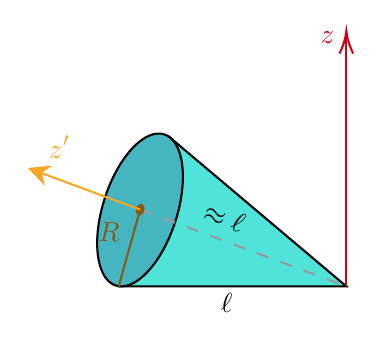
\begin{tikzpicture}[x=0.75pt,y=0.75pt,yscale=-1,xscale=1]
		%uncomment if require: \path (0,156); %set diagram left start at 0, and has height of 156
		
		%Straight Lines [id:da46986834064120264] 
		\draw [fill={rgb, 255:red, 80; green, 227; blue, 217 }  ,fill opacity=1 ]   (88.98,62.4) -- (175,135) -- (65,135) ;
		%Shape: Ellipse [id:dp021793458814799216] 
		\draw  [fill={rgb, 255:red, 69; green, 181; blue, 194 }  ,fill opacity=1 ] (87.6,61.89) .. controls (96.88,65.32) and (99.03,84.35) .. (92.4,104.39) .. controls (85.77,124.44) and (72.87,137.91) .. (63.59,134.48) .. controls (54.31,131.05) and (52.16,112.03) .. (58.79,91.98) .. controls (65.42,71.94) and (78.32,58.47) .. (87.6,61.89) -- cycle ;
		%Straight Lines [id:da6443901401504621] 
		\draw [color={rgb, 255:red, 208; green, 2; blue, 27 }  ,draw opacity=1 ]   (175,135) -- (175,13.91) ;
		\draw [shift={(175,11.91)}, rotate = 90] [color={rgb, 255:red, 208; green, 2; blue, 27 }  ,draw opacity=1 ][line width=0.75]    (10.93,-3.29) .. controls (6.95,-1.4) and (3.31,-0.3) .. (0,0) .. controls (3.31,0.3) and (6.95,1.4) .. (10.93,3.29)   ;
		%Straight Lines [id:da7224554163863225] 
		\draw [color={rgb, 255:red, 134; green, 90; blue, 17 }  ,draw opacity=1 ]   (75.6,98.19) -- (65.29,135.06) ;
		%Straight Lines [id:da17713702184878055] 
		\draw [color={rgb, 255:red, 155; green, 155; blue, 155 }  ,draw opacity=1 ] [dash pattern={on 4.5pt off 4.5pt}]  (75.65,98.03) -- (175,135) ;
		%Shape: Ellipse [id:dp08811005725484056] 
		\draw  [draw opacity=0][fill={rgb, 255:red, 134; green, 90; blue, 17 }  ,fill opacity=1 ] (76.58,95.22) .. controls (77.61,95.6) and (78.04,97.17) .. (77.52,98.73) .. controls (77.01,100.28) and (75.75,101.23) .. (74.71,100.85) .. controls (73.68,100.47) and (73.26,98.9) .. (73.77,97.34) .. controls (74.29,95.79) and (75.54,94.84) .. (76.58,95.22) -- cycle ;
		%Straight Lines [id:da7907122971129069] 
		\draw [color={rgb, 255:red, 245; green, 166; blue, 35 }  ,draw opacity=1 ]   (24.34,79) -- (75.65,98.03) ;
		\draw [shift={(21.52,77.95)}, rotate = 20.36] [fill={rgb, 255:red, 245; green, 166; blue, 35 }  ,fill opacity=1 ][line width=0.08]  [draw opacity=0] (10.72,-5.15) -- (0,0) -- (10.72,5.15) -- (7.12,0) -- cycle    ;
		
		% Text Node
		\draw (30,61) node [anchor=north west][inner sep=0.75pt]  [color={rgb, 255:red, 245; green, 166; blue, 35 }  ,opacity=1 ] [align=left] {$\displaystyle z'$};
		% Text Node
		\draw (161,10.86) node [anchor=north west][inner sep=0.75pt]  [color={rgb, 255:red, 208; green, 2; blue, 27 }  ,opacity=1 ] [align=left] {$\displaystyle z$};
		% Text Node
		\draw (54,102.58) node [anchor=north west][inner sep=0.75pt]  [color={rgb, 255:red, 134; green, 90; blue, 17 }  ,opacity=1 ] [align=left] {$\displaystyle R$};
		% Text Node
		\draw (113,137) node [anchor=north west][inner sep=0.75pt]   [align=left] {$\displaystyle \ell $};
		% Text Node
		\draw (107.84,92.38) node [anchor=north west][inner sep=0.75pt]  [rotate=-20] [align=left] {$\displaystyle \approx \ell $};
	\end{tikzpicture}
\end{figure}

Ya que \(\ell \gg R\), podemos considerar que la distancia entre el centro de la base y el origen del plano es \(\approx \ell\). Por ende, el cono tendrá un volumen de
\begin{equation}
	V \approx \frac{1}{3}\pi R^2 \ell
\end{equation}
y una densidad constante y homogénea
\begin{equation}
	\rho = \frac{m}{V} \approx \frac{3 m}{\pi R^2 \ell}
\end{equation}
%
%El centro de masa del cono estará, por simetría, sobre su eje central \(z'\), por lo que para encontrar su posición dentro del eje solo necesitamos 
%\begin{equation}
%	\mathbf{y}_{\mathrm{CM}} = \hat{\mathbf{z}}'\frac{1}{V} \int_{0}^{\ell} x A(x) \, dx = \frac{3}{4}\ell \,\hat{\mathbf{z}}' \approx \frac{3}{4}\ell\,\rhat
%\end{equation}
\begin{figure}[h!]
	\centering
	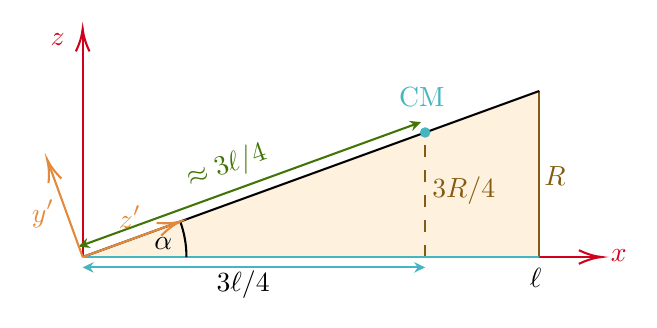
\begin{tikzpicture}[x=0.75pt,y=0.75pt,yscale=-1,xscale=1]
		%uncomment if require: \path (0,156); %set diagram left start at 0, and has height of 156
		
		%Straight Lines [id:da6161622843204072] 
		\draw [draw opacity=0][fill={rgb, 255:red, 245; green, 166; blue, 35 }  ,fill opacity=0.15 ]   (85,121) -- (305,121) -- (305,41) -- cycle ;
		%Straight Lines [id:da11763639827021244] 
		\draw [color={rgb, 255:red, 208; green, 2; blue, 27 }  ,draw opacity=1 ]   (85,121) -- (333,121) ;
		\draw [shift={(335,121)}, rotate = 180] [color={rgb, 255:red, 208; green, 2; blue, 27 }  ,draw opacity=1 ][line width=0.75]    (10.93,-3.29) .. controls (6.95,-1.4) and (3.31,-0.3) .. (0,0) .. controls (3.31,0.3) and (6.95,1.4) .. (10.93,3.29)   ;
		%Straight Lines [id:da5149621051786881] 
		\draw [color={rgb, 255:red, 134; green, 90; blue, 17 }  ,draw opacity=1 ]   (305,121) -- (305,41) ;
		%Straight Lines [id:da4780316742320835] 
		\draw    (305,41) -- (85,121) ;
		%Straight Lines [id:da7251070703567969] 
		\draw [color={rgb, 255:red, 208; green, 2; blue, 27 }  ,draw opacity=1 ]   (85,121) -- (85,13) ;
		\draw [shift={(85,11)}, rotate = 90] [color={rgb, 255:red, 208; green, 2; blue, 27 }  ,draw opacity=1 ][line width=0.75]    (10.93,-3.29) .. controls (6.95,-1.4) and (3.31,-0.3) .. (0,0) .. controls (3.31,0.3) and (6.95,1.4) .. (10.93,3.29)   ;
		%Straight Lines [id:da008603182697215384] 
		\draw [color={rgb, 255:red, 65; green, 117; blue, 5 }  ,draw opacity=1 ]   (245.18,57.03) -- (85.82,114.97) ;
		\draw [shift={(83,116)}, rotate = 340.02] [fill={rgb, 255:red, 65; green, 117; blue, 5 }  ,fill opacity=1 ][line width=0.08]  [draw opacity=0] (5.36,-2.57) -- (0,0) -- (5.36,2.57) -- (3.56,0) -- cycle    ;
		\draw [shift={(248,56)}, rotate = 160.02] [fill={rgb, 255:red, 65; green, 117; blue, 5 }  ,fill opacity=1 ][line width=0.08]  [draw opacity=0] (5.36,-2.57) -- (0,0) -- (5.36,2.57) -- (3.56,0) -- cycle    ;
		%Straight Lines [id:da99311338027557] 
		\draw [color={rgb, 255:red, 134; green, 90; blue, 17 }  ,draw opacity=1 ] [dash pattern={on 4.5pt off 4.5pt}]  (250,121) -- (250,61) ;
		%Shape: Circle [id:dp9801749765517975] 
		\draw  [color={rgb, 255:red, 69; green, 181; blue, 194 }  ,draw opacity=1 ][fill={rgb, 255:red, 69; green, 181; blue, 194 }  ,fill opacity=1 ] (252,61) .. controls (252,59.9) and (251.1,59) .. (250,59) .. controls (248.9,59) and (248,59.9) .. (248,61) .. controls (248,62.1) and (248.9,63) .. (250,63) .. controls (251.1,63) and (252,62.1) .. (252,61) -- cycle ;
		%Straight Lines [id:da7150964315309531] 
		\draw [color={rgb, 255:red, 69; green, 181; blue, 194 }  ,draw opacity=1 ]   (305,121) -- (85,121) ;
		%Straight Lines [id:da25391155999585835] 
		\draw [color={rgb, 255:red, 69; green, 181; blue, 194 }  ,draw opacity=1 ]   (247,126) -- (88,126) ;
		\draw [shift={(85,126)}, rotate = 360] [fill={rgb, 255:red, 69; green, 181; blue, 194 }  ,fill opacity=1 ][line width=0.08]  [draw opacity=0] (5.36,-2.57) -- (0,0) -- (5.36,2.57) -- (3.56,0) -- cycle    ;
		\draw [shift={(250,126)}, rotate = 180] [fill={rgb, 255:red, 69; green, 181; blue, 194 }  ,fill opacity=1 ][line width=0.08]  [draw opacity=0] (5.36,-2.57) -- (0,0) -- (5.36,2.57) -- (3.56,0) -- cycle    ;
		%Shape: Arc [id:dp7105647894433695] 
		\draw  [draw opacity=0] (132,103.89) .. controls (133.94,109.23) and (135,114.99) .. (135,121) -- (85,121) -- cycle ; \draw [color={rgb, 255:red, 0; green, 0; blue, 0 }  ,draw opacity=1 ]   (132,103.89) .. controls (133.94,109.23) and (135,114.99) .. (135,121) ;  
		%Straight Lines [id:da13574596092560787] 
		\draw [color={rgb, 255:red, 226; green, 137; blue, 59 }  ,draw opacity=1 ]   (85,121) -- (130.12,104.58) ;
		\draw [shift={(132,103.89)}, rotate = 160] [color={rgb, 255:red, 226; green, 137; blue, 59 }  ,draw opacity=1 ][line width=0.75]    (10.93,-3.29) .. controls (6.95,-1.4) and (3.31,-0.3) .. (0,0) .. controls (3.31,0.3) and (6.95,1.4) .. (10.93,3.29)   ;
		%Straight Lines [id:da5687635510746675] 
		\draw [color={rgb, 255:red, 226; green, 137; blue, 59 }  ,draw opacity=1 ]   (85,121) -- (68.58,75.88) ;
		\draw [shift={(67.89,74)}, rotate = 70] [color={rgb, 255:red, 226; green, 137; blue, 59 }  ,draw opacity=1 ][line width=0.75]    (10.93,-3.29) .. controls (6.95,-1.4) and (3.31,-0.3) .. (0,0) .. controls (3.31,0.3) and (6.95,1.4) .. (10.93,3.29)   ;
		
		% Text Node
		\draw (148,126) node [anchor=north west][inner sep=0.75pt]   [align=left] {$\displaystyle 3\ell /4$};
		% Text Node
		\draw (131.62,76.86) node [anchor=north west][inner sep=0.75pt]  [color={rgb, 255:red, 65; green, 117; blue, 5 }  ,opacity=1 ,rotate=-340] [align=left] {$\displaystyle \approx 3\ell /4$};
		% Text Node
		\draw (306,76) node [anchor=north west][inner sep=0.75pt]  [color={rgb, 255:red, 134; green, 90; blue, 17 }  ,opacity=1 ] [align=left] {$\displaystyle R$};
		% Text Node
		\draw (338,116) node [anchor=north west][inner sep=0.75pt]  [color={rgb, 255:red, 208; green, 2; blue, 27 }  ,opacity=1 ] [align=left] {$\displaystyle x$};
		% Text Node
		\draw (68,12) node [anchor=north west][inner sep=0.75pt]  [color={rgb, 255:red, 208; green, 2; blue, 27 }  ,opacity=1 ] [align=left] {$\displaystyle z$};
		% Text Node
		\draw (236,38) node [anchor=north west][inner sep=0.75pt]  [color={rgb, 255:red, 69; green, 181; blue, 194 }  ,opacity=1 ] [align=left] {$\displaystyle \mathrm{CM}$};
		% Text Node
		\draw (252,81) node [anchor=north west][inner sep=0.75pt]  [color={rgb, 255:red, 134; green, 90; blue, 17 }  ,opacity=1 ] [align=left] {$\displaystyle 3R/4$};
		% Text Node
		\draw (299,125) node [anchor=north west][inner sep=0.75pt]   [align=left] {$\displaystyle \ell $};
		% Text Node
		\draw (118,110) node [anchor=north west][inner sep=0.75pt]   [align=left] {$\displaystyle \alpha $};
		% Text Node
		\draw (101,95) node [anchor=north west][inner sep=0.75pt]  [color={rgb, 255:red, 226; green, 137; blue, 59 }  ,opacity=1 ] [align=left] {$\displaystyle z'$};
		% Text Node
		\draw (59,92) node [anchor=north west][inner sep=0.75pt]  [color={rgb, 255:red, 226; green, 137; blue, 59 }  ,opacity=1 ] [align=left] {$\displaystyle y'$};		
	\end{tikzpicture}
\end{figure}

Consideremos los ángulos de Euler para un sistema de coordenadas \(Y,Z,Z'\) con ángulos \((\psi, \theta, \varphi)\) que representan, respectivamente, la elevación respecto del plano \(XY\), la rotación alrededor del eje central del plano, y la rotación del cono sobre su propio eje central.


\begin{figure}[h!]
	\centering
	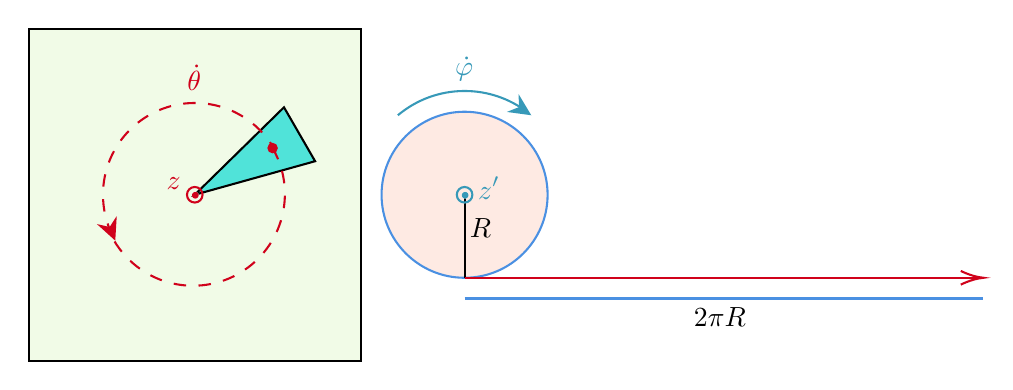
\begin{tikzpicture}[x=0.75pt,y=0.75pt,yscale=-1,xscale=1]
		%uncomment if require: \path (0,200); %set diagram left start at 0, and has height of 200
		
		%Shape: Square [id:dp33761967112596813] 
		\draw  [fill={rgb, 255:red, 184; green, 233; blue, 134 }  ,fill opacity=0.2 ] (25,25) -- (185,25) -- (185,185) -- (25,185) -- cycle ;
		%Shape: Triangle [id:dp5404121407269246] 
		\draw  [fill={rgb, 255:red, 80; green, 227; blue, 217 }  ,fill opacity=1 ] (105,105) -- (147.99,62.86) -- (162.99,88.84) -- cycle ;
		%Shape: Circle [id:dp5440458563261413] 
		\draw  [color={rgb, 255:red, 208; green, 2; blue, 27 }  ,draw opacity=1 ][fill={rgb, 255:red, 208; green, 2; blue, 27 }  ,fill opacity=1 ] (144.5,82.5) .. controls (144.5,81.4) and (143.6,80.5) .. (142.5,80.5) .. controls (141.4,80.5) and (140.5,81.4) .. (140.5,82.5) .. controls (140.5,83.6) and (141.4,84.5) .. (142.5,84.5) .. controls (143.6,84.5) and (144.5,83.6) .. (144.5,82.5) -- cycle ;
		%Shape: Arc [id:dp1556557739667963] 
		\draw  [draw opacity=0][dash pattern={on 4.5pt off 4.5pt}] (66.7,127.11) .. controls (62.94,120.61) and (60.78,113.06) .. (60.78,105) .. controls (60.78,80.58) and (80.58,60.78) .. (105,60.78) .. controls (121.37,60.78) and (135.65,69.67) .. (143.3,82.89) -- (105,105) -- cycle ; \draw [color={rgb, 255:red, 208; green, 2; blue, 27 }  ,draw opacity=1 ][dash pattern={on 4.5pt off 4.5pt}] [dash pattern={on 4.5pt off 4.5pt}]  (65.26,124.42) .. controls (62.39,118.56) and (60.78,111.97) .. (60.78,105) .. controls (60.78,80.58) and (80.58,60.78) .. (105,60.78) .. controls (121.37,60.78) and (135.65,69.67) .. (143.3,82.89) ;  \draw [shift={(66.7,127.11)}, rotate = 247.75] [fill={rgb, 255:red, 208; green, 2; blue, 27 }  ,fill opacity=1 ][dash pattern={on 3.49pt off 4.5pt}][line width=0.08]  [draw opacity=0] (10.72,-5.15) -- (0,0) -- (10.72,5.15) -- (7.12,0) -- cycle    ;
		%Shape: Arc [id:dp3411022668634043] 
		\draw  [draw opacity=0][dash pattern={on 4.5pt off 4.5pt}] (142.5,82.5) .. controls (146.26,89) and (148.42,96.56) .. (148.42,104.61) .. controls (148.42,129.03) and (128.62,148.83) .. (104.2,148.83) .. controls (87.83,148.83) and (73.54,139.94) .. (65.9,126.73) -- (104.2,104.61) -- cycle ; \draw [color={rgb, 255:red, 208; green, 2; blue, 27 }  ,draw opacity=1 ][dash pattern={on 4.5pt off 4.5pt}] [dash pattern={on 4.5pt off 4.5pt}]  (142.5,82.5) .. controls (146.26,89) and (148.42,96.56) .. (148.42,104.61) .. controls (148.42,129.03) and (128.62,148.83) .. (104.2,148.83) .. controls (87.83,148.83) and (73.54,139.94) .. (65.9,126.73) ;  
		%Shape: Circle [id:dp42284116385241155] 
		\draw  [color={rgb, 255:red, 74; green, 144; blue, 226 }  ,draw opacity=1 ][fill={rgb, 255:red, 252; green, 171; blue, 142 }  ,fill opacity=0.25 ] (195,105) .. controls (195,82.91) and (212.91,65) .. (235,65) .. controls (257.09,65) and (275,82.91) .. (275,105) .. controls (275,127.09) and (257.09,145) .. (235,145) .. controls (212.91,145) and (195,127.09) .. (195,105) -- cycle ;
		%Straight Lines [id:da22599383595059785] 
		\draw    (235,145) -- (235,105) ;
		%Straight Lines [id:da8540039123821289] 
		\draw [color={rgb, 255:red, 74; green, 144; blue, 226 }  ,draw opacity=1 ]   (235,155) -- (485,155) ;
		%Straight Lines [id:da7553104285096213] 
		\draw [color={rgb, 255:red, 208; green, 2; blue, 27 }  ,draw opacity=1 ]   (235,145) -- (483,145) ;
		\draw [shift={(485,145)}, rotate = 180] [color={rgb, 255:red, 208; green, 2; blue, 27 }  ,draw opacity=1 ][line width=0.75]    (10.93,-3.29) .. controls (6.95,-1.4) and (3.31,-0.3) .. (0,0) .. controls (3.31,0.3) and (6.95,1.4) .. (10.93,3.29)   ;
		%Shape: Circle [id:dp5853021214021392] 
		\path  [shading=_y4oyjsov0,_t5mdhtxnp,path fading= _bcb2u9fkc ,fading transform={xshift=2}] (101.25,105) .. controls (101.25,102.93) and (102.93,101.25) .. (105,101.25) .. controls (107.07,101.25) and (108.75,102.93) .. (108.75,105) .. controls (108.75,107.07) and (107.07,108.75) .. (105,108.75) .. controls (102.93,108.75) and (101.25,107.07) .. (101.25,105) -- cycle ; % for fading 
		\draw  [color={rgb, 255:red, 208; green, 2; blue, 27 }  ,draw opacity=1 ] (101.25,105) .. controls (101.25,102.93) and (102.93,101.25) .. (105,101.25) .. controls (107.07,101.25) and (108.75,102.93) .. (108.75,105) .. controls (108.75,107.07) and (107.07,108.75) .. (105,108.75) .. controls (102.93,108.75) and (101.25,107.07) .. (101.25,105) -- cycle ; % for border 
		
		%Shape: Arc [id:dp6768692699740413] 
		\draw  [draw opacity=0] (202.86,66.7) .. controls (211.55,59.4) and (222.76,55) .. (235,55) .. controls (247.24,55) and (258.45,59.4) .. (267.14,66.7) -- (235,105) -- cycle ; \draw [color={rgb, 255:red, 55; green, 153; blue, 184 }  ,draw opacity=1 ]   (202.86,66.7) .. controls (211.55,59.4) and (222.76,55) .. (235,55) .. controls (246.2,55) and (256.54,58.68) .. (264.87,64.9) ; \draw [shift={(267.14,66.7)}, rotate = 213.41] [fill={rgb, 255:red, 55; green, 153; blue, 184 }  ,fill opacity=1 ][line width=0.08]  [draw opacity=0] (10.72,-5.15) -- (0,0) -- (10.72,5.15) -- (7.12,0) -- cycle    ; 
		%Shape: Circle [id:dp03854455384046296] 
		\path  [shading=_6rp8budzf,_86h7qoix5,path fading= _okjtkvlfh ,fading transform={xshift=2}] (231.25,105) .. controls (231.25,102.93) and (232.93,101.25) .. (235,101.25) .. controls (237.07,101.25) and (238.75,102.93) .. (238.75,105) .. controls (238.75,107.07) and (237.07,108.75) .. (235,108.75) .. controls (232.93,108.75) and (231.25,107.07) .. (231.25,105) -- cycle ; % for fading 
		\draw  [color={rgb, 255:red, 55; green, 153; blue, 184 }  ,draw opacity=1 ] (231.25,105) .. controls (231.25,102.93) and (232.93,101.25) .. (235,101.25) .. controls (237.07,101.25) and (238.75,102.93) .. (238.75,105) .. controls (238.75,107.07) and (237.07,108.75) .. (235,108.75) .. controls (232.93,108.75) and (231.25,107.07) .. (231.25,105) -- cycle ; % for border 
		
		
		% Text Node
		\draw (236,115) node [anchor=north west][inner sep=0.75pt]   [align=left] {$\displaystyle R$};
		% Text Node
		\draw (344,158) node [anchor=north west][inner sep=0.75pt]   [align=left] {$\displaystyle 2\pi R$};
		% Text Node
		\draw (100,41) node [anchor=north west][inner sep=0.75pt]  [color={rgb, 255:red, 208; green, 2; blue, 27 }  ,opacity=1 ] [align=left] {$\displaystyle \dot{\theta }$};
		% Text Node
		\draw (229,37) node [anchor=north west][inner sep=0.75pt]  [color={rgb, 255:red, 55; green, 153; blue, 184 }  ,opacity=1 ] [align=left] {$\displaystyle \dot{\varphi }$};
		% Text Node
		\draw (90,95) node [anchor=north west][inner sep=0.75pt]  [color={rgb, 255:red, 208; green, 2; blue, 27 }  ,opacity=1 ] [align=left] {$\displaystyle z$};
		% Text Node
		\draw (240,95) node [anchor=north west][inner sep=0.75pt]  [color={rgb, 255:red, 55; green, 153; blue, 184 }  ,opacity=1 ] [align=left] {$\displaystyle z'$};
	\end{tikzpicture}
\end{figure}

Tendremos los siguientes \textit{constraints}:
\begin{enumerate}
	\item El cono reposa sobre el plano \(XY\), por lo que:
	\begin{equation}
		\psi = \alpha = \mathrm{const.} ~~~ \Rightarrow ~~~ \dot{\psi} = 0
	\end{equation}
	\item Condición de rodamiento:
	\begin{equation}
		\ell \theta = R \varphi ~~~ \Rightarrow ~~~ \dot{\varphi} = \frac{\ell}{R} \dot{\theta} \label{equiv_angulos}
	\end{equation}
\end{enumerate}

Por lo que el vector de velocidad angular será:
\begin{equation}
	\Omega =  \dot{\theta}\zhat + \dot{\psi}\yhat + \dot{\varphi}\zhat' = \dot{\theta}\zhat + \frac{\ell}{R} \dot{\theta}\zhat'
\end{equation}
Pero, ya que \(\ell \gg R\), podemos considerar que \(\zhat \approx \yhat'\). Por lo tanto, en el sistema de coordenadas del cono tendremos que:
\begin{equation}
	\Omega \approx \dot{\theta}\yhat' + \frac{\ell}{R} \dot{\theta}\zhat'
\end{equation}
%Si consideramos que el centro de masa tiene una velocidad \(\Vv_\mathrm{CM}\), y que orbita el origen con velocidad angular \(\dot{\theta}\):
%\begin{equation}
%	|\Vv_\mathrm{CM}| = \frac{3\ell}{4} \dot{\theta}
%\end{equation}
%Y tomamos que el cono rota sobre su eje \(z'\) con velocidad angular \(-\dot{\varphi}\) (negativo porque va en sentido horario), donde tenemos la equivalencia:
%\begin{align}
%	\frac{3\ell}{4} \theta &= \frac{3R}{4} \varphi \nonumber\\
%	\Rightarrow \theta &= \frac{R}{\ell} \varphi \label{equiv_angulos}
%\end{align}

Como el eje de rotación del cono coincide con su eje central, podemos calcular el tensor de inercia en el marco en reposo como:
\begin{align}
	\hat{I} &= \int dV \, \rho(\rv) \, (\delta_{jk} r^2 - r_{j} r_{k}) \nonumber\\
	&= \frac{3}{20} m \begin{pmatrix}
		4 l^2+R^2 & 0 & 0 \\
		0 & 4 l^2+R^2 & 0 \\
		0 & 0 & 2 R^2
	\end{pmatrix}
\end{align}
%Y luego, utilizando la matriz de rotación para pasar del sistema en reposo al sistema del laboratorio:
%\begin{equation*}
%	\hat{R} = \begin{pmatrix}
%		\cos(\theta) & -\sin(\theta) & 0\\
%		\sin(\theta) &  \cos(\theta) & 0\\
%		0            & 0              & 1
%	\end{pmatrix} \begin{pmatrix}
%		1 & 0                           & 0                              \\
%		0 & \cos(\frac{\pi}{2} - \alpha) & -\sin(\frac{\pi}{2} - \alpha) \\
%		0 & \sin(\frac{\pi}{2} - \alpha) &  \cos(\frac{\pi}{2} - \alpha)
%	\end{pmatrix}
%\end{equation*}
%donde \(\alpha = \arctan(\frac{R}{\ell})\). Pero \(\alpha \approx 0\), por lo que la matriz de rotación, el tensor de inercia, y el vector de velocidad angular en coordenadas del laboratorio serán
%\begin{equation}
%	\Rightarrow \hat{R} \approx \begin{pmatrix}
%		\cos(\theta) & 0 &  \sin(\theta) \\
%		\sin(\theta) & 0 & -\cos(\theta) \\
%		0            & 1 & 0                            
%	\end{pmatrix}
%\end{equation}
%\begin{equation}
%	\Rightarrow \hat{I} \rightarrow \frac{3}{20} m \begin{pmatrix}
%			4 l^2+R^2 & 0 & 0 \\
%			0 & 2 R^2 & 0 \\
%			0 & 0 & 4 l^2+R^2
%	\end{pmatrix}
%\end{equation}
%\begin{equation}
%	\Rightarrow \dot{\vec{\varphi}} \rightarrow \begin{pmatrix}
%			\dot{\varphi } \sin (\theta ) \\
%			- \dot{\varphi } \cos (\theta ) \\
%			0
%	\end{pmatrix}
%\end{equation}
La energía cinética rotacional queda entonces como
\begin{equation}
	T = \frac{1}{2}I_{jk} \Omega_{j}(t) \Omega_{k}(t) = \frac{1}{2}\Omega^{T}\hat{I}\Omega = \frac{3}{40} m \left(6 \ell^2+R^2\right) \dot{\theta }^2
\end{equation}
Finalmente el lagrangiano, y asumiendo que el campo potencial es nulo
\begin{equation}
	L = T - U = \frac{3}{40} m \left(6 \ell^2+R^2\right) \dot{\theta }^2
\end{equation}
De aquí se desprende que \(\theta\) es una coordenada cíclica. Si consideramos que el plano sobre el cual reposa el cono y el punto fijo de su cúspide están únicamente definidos, tendremos solo 2 simetrías para el lagrangiano:
\begin{align}
	\theta &\rightarrow \theta + \epsilon \nonumber\\
	Q_\theta = \pd{L}{\dot{\theta}} &= \frac{3}{20} m \left(6 \ell^2+R^2\right) \dot{\theta }\\
	t &\rightarrow t + \epsilon \nonumber\\
	E &= \frac{3}{40} m \left(6 \ell^2+R^2\right) \dot{\theta }^2
\end{align}
% % % % % % % % % % % % % % % % % % % % % % % % % % % % % % % % % % % % % % % % % % % % % % % % % % % % % %

\begin{enumerate}
	\item[\textbf{b.}] Write out the Euler-Lagrange equations and integrate	them. You may use integrals of motion to find the trajectories.
\end{enumerate}

Ya que hay solo una variable, la ecuación de Euler-Lagrange:
\begin{align*}
	\pd{L}{\theta} - \td{}{t}\left(\pd{L}{\dot{\theta}}\right) &= 0 \\
	\Rightarrow \frac{3}{20} m \left(6 \ell^2+R^2\right) \ddot{\theta } &= 0
\end{align*}
\begin{equation}
	\Rightarrow\ddot{\theta} = 0
\end{equation}
Para encontrar la trayectoria integramos \(\ddot{\theta}\)
\begin{equation}
	\theta(t) = \omega_{0} t + \theta_{0}
\end{equation}
Consideramos al centro de masa como punto a seguir, el cual se encuentra a una posición:
\begin{equation*}
	z'_{\mathrm{CM}} = \wfrac{\int _0^l\int _0^{R z / l}\int _0^{2 \pi }z \, r d\theta drdz}{\int _0^l\int _0^{R z / l}\int _0^{2 \pi }rd\theta drdz} = \frac{3}{4}\ell
\end{equation*}
Y, como \(\zhat' \approx \rhat\):
\begin{equation}
	r_{\mathrm{CM}} \approx \frac{3}{4}\ell
\end{equation}
Incluyendo entonces el movimiento rotacional:
\begin{equation}
	\left. \begin{matrix}
		x_{\mathrm{CM}}(t) = \dfrac{3}{4}\ell \cos(\omega_{0} t + \theta_{0})\vspace{5mm}\\
		y_{\mathrm{CM}}(t) = \dfrac{3}{4}\ell \sin(\omega_{0} t + \theta_{0})
	\end{matrix}\right\rbrace
\end{equation}
Es decir, una simple órbita circular.

%%%%%%%%%%%%%%%%%%%%%%%%%%%%%%%%%%%%%%%%%%%%%%%%%%%%%%%%%%%%%%%%%%%%%%%%%%%%%%%%%%%%%%%%%%%%%%%%%%%%%%%%%%%

\section{Pregunta 2}
The electrons are emitted isotropically with constant energy \(E\) at the point \(A\). We need to create the central potential \(U(r)\) that will focus them at the point \(F\) located at some distance. The center of the field (point \(O\)) is located on the line connecting the points \(A\) and \(F\), at distances \(R_{1}\) and \(R_{2}\) from them, respectively. For the sake of simplicity, You may assume that \(R_{1} = R_{2} = R\), and that the potential vanishes at distances \(r > R\) from the point \(O\) (the so-called ``\textit{Maxwell's fish-eye configuration}'').

\begin{figure}[h!]
	\centering
	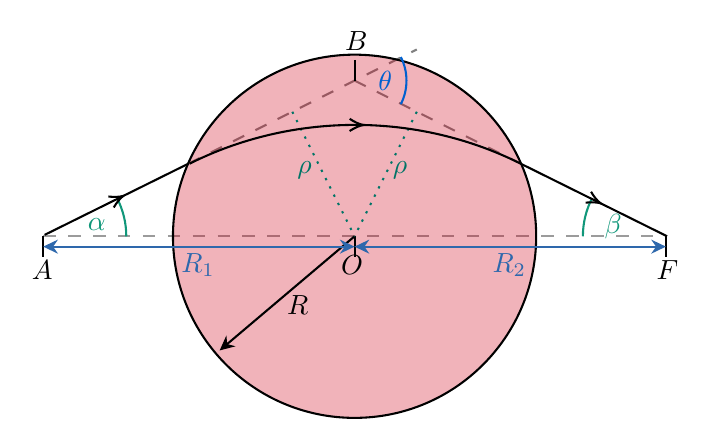
\begin{tikzpicture}[x=0.75pt,y=0.75pt,yscale=-1,xscale=1]
		%uncomment if require: \path (0,220); %set diagram left start at 0, and has height of 220
		
		%Straight Lines [id:da22896508470176902] 
		\draw [color={rgb, 255:red, 128; green, 128; blue, 128 }  ,draw opacity=1 ] [dash pattern={on 4.5pt off 4.5pt}]  (115,77.5) -- (225,22.5) ;
		%Straight Lines [id:da4252899641944393] 
		\draw [color={rgb, 255:red, 128; green, 128; blue, 128 }  ,draw opacity=1 ] [dash pattern={on 4.5pt off 4.5pt}]  (195,37.5) -- (275,77.5) ;
		%Straight Lines [id:da41128984149043146] 
		\draw [color={rgb, 255:red, 155; green, 155; blue, 155 }  ,draw opacity=1 ] [dash pattern={on 4.5pt off 4.5pt}]  (45,112.5) -- (345,112.5) ;
		%Shape: Circle [id:dp6953915635540854] 
		\draw  [fill={rgb, 255:red, 208; green, 2; blue, 27 }  ,fill opacity=0.3 ] (107.5,112.5) .. controls (107.5,64.18) and (146.68,25) .. (195,25) .. controls (243.32,25) and (282.5,64.18) .. (282.5,112.5) .. controls (282.5,160.82) and (243.32,200) .. (195,200) .. controls (146.68,200) and (107.5,160.82) .. (107.5,112.5) -- cycle ;
		%Straight Lines [id:da6484289282974143] 
		\draw    (195,112.5) -- (195,122.5) ;
		%Straight Lines [id:da19759329821093452] 
		\draw    (45,112.5) -- (45,122.5) ;
		%Straight Lines [id:da5791899844416095] 
		\draw    (345,112.5) -- (345,122.5) ;
		%Shape: Arc [id:dp2314315416020447] 
		\draw  [draw opacity=0] (217.28,26.15) .. controls (219.02,29.55) and (220,33.41) .. (220,37.5) .. controls (220,41.59) and (219.02,45.45) .. (217.28,48.85) -- (195,37.5) -- cycle ; \draw  [color={rgb, 255:red, 0; green, 96; blue, 207 }  ,draw opacity=1 ] (217.28,26.15) .. controls (219.02,29.55) and (220,33.41) .. (220,37.5) .. controls (220,41.59) and (219.02,45.45) .. (217.28,48.85) ;  
		%Shape: Arc [id:dp397979074527137] 
		\draw  [draw opacity=0] (80.65,94.34) .. controls (83.43,99.79) and (85,105.96) .. (85,112.5) -- (45,112.5) -- cycle ; \draw  [color={rgb, 255:red, 17; green, 151; blue, 122 }  ,draw opacity=1 ] (80.65,94.34) .. controls (83.43,99.79) and (85,105.96) .. (85,112.5) ;  
		%Shape: Arc [id:dp6383682171746863] 
		\draw  [draw opacity=0] (309.35,94.34) .. controls (306.57,99.79) and (305,105.96) .. (305,112.5) -- (345,112.5) -- cycle ; \draw  [color={rgb, 255:red, 17; green, 151; blue, 122 }  ,draw opacity=1 ] (309.35,94.34) .. controls (306.57,99.79) and (305,105.96) .. (305,112.5) ;  
		%Straight Lines [id:da8252860520998729] 
		\draw    (195,112.5) -- (132.29,165.56) ;
		\draw [shift={(130,167.5)}, rotate = 319.76] [fill={rgb, 255:red, 0; green, 0; blue, 0 }  ][line width=0.08]  [draw opacity=0] (7.14,-3.43) -- (0,0) -- (7.14,3.43) -- (4.74,0) -- cycle    ;
		%Straight Lines [id:da9224386725643036] 
		\draw [color={rgb, 255:red, 46; green, 104; blue, 172 }  ,draw opacity=1 ]   (48,117.5) -- (192,117.5) ;
		\draw [shift={(195,117.5)}, rotate = 180] [fill={rgb, 255:red, 46; green, 104; blue, 172 }  ,fill opacity=1 ][line width=0.08]  [draw opacity=0] (7.14,-3.43) -- (0,0) -- (7.14,3.43) -- (4.74,0) -- cycle    ;
		\draw [shift={(45,117.5)}, rotate = 0] [fill={rgb, 255:red, 46; green, 104; blue, 172 }  ,fill opacity=1 ][line width=0.08]  [draw opacity=0] (7.14,-3.43) -- (0,0) -- (7.14,3.43) -- (4.74,0) -- cycle    ;
		%Straight Lines [id:da26224741793239914] 
		\draw [color={rgb, 255:red, 46; green, 104; blue, 172 }  ,draw opacity=1 ]   (198,117.5) -- (342,117.5) ;
		\draw [shift={(345,117.5)}, rotate = 180] [fill={rgb, 255:red, 46; green, 104; blue, 172 }  ,fill opacity=1 ][line width=0.08]  [draw opacity=0] (7.14,-3.43) -- (0,0) -- (7.14,3.43) -- (4.74,0) -- cycle    ;
		\draw [shift={(195,117.5)}, rotate = 0] [fill={rgb, 255:red, 46; green, 104; blue, 172 }  ,fill opacity=1 ][line width=0.08]  [draw opacity=0] (7.14,-3.43) -- (0,0) -- (7.14,3.43) -- (4.74,0) -- cycle    ;
		%Straight Lines [id:da516054537434487] 
		\draw    (195,27.5) -- (195,37.5) ;
		%Straight Lines [id:da5249287860167562] 
		\draw [color={rgb, 255:red, 0; green, 116; blue, 102 }  ,draw opacity=1 ] [dash pattern={on 0.84pt off 2.51pt}]  (165,52.5) -- (195,112.5) ;
		%Straight Lines [id:da7311496936773492] 
		\draw    (275,77.5) -- (345.56,112.5) ;
		\draw [shift={(313.5,96.6)}, rotate = 206.38] [color={rgb, 255:red, 0; green, 0; blue, 0 }  ][line width=0.75]    (6.56,-2.94) .. controls (4.17,-1.38) and (1.99,-0.4) .. (0,0) .. controls (1.99,0.4) and (4.17,1.38) .. (6.56,2.94)   ;
		%Straight Lines [id:da8895849006345163] 
		\draw    (45.65,111.84) -- (115,77.5) ;
		\draw [shift={(83.55,93.07)}, rotate = 153.66] [color={rgb, 255:red, 0; green, 0; blue, 0 }  ][line width=0.75]    (6.56,-2.94) .. controls (4.17,-1.38) and (1.99,-0.4) .. (0,0) .. controls (1.99,0.4) and (4.17,1.38) .. (6.56,2.94)   ;
		%Straight Lines [id:da2582455789509056] 
		\draw [color={rgb, 255:red, 0; green, 116; blue, 102 }  ,draw opacity=1 ] [dash pattern={on 0.84pt off 2.51pt}]  (225,52.5) -- (195,112.5) ;
		%Curve Lines [id:da38594122551837484] 
		\draw    (115.56,77.5) .. controls (165,52.75) and (225,52.5) .. (275,77.5) ;
		\draw [shift={(199.18,58.89)}, rotate = 180.32] [color={rgb, 255:red, 0; green, 0; blue, 0 }  ][line width=0.75]    (6.56,-2.94) .. controls (4.17,-1.38) and (1.99,-0.4) .. (0,0) .. controls (1.99,0.4) and (4.17,1.38) .. (6.56,2.94)   ;
		
		% Text Node
		\draw (187,120.5) node [anchor=north west][inner sep=0.75pt]   [align=left] {$\displaystyle O$};
		% Text Node
		\draw (110,119.5) node [anchor=north west][inner sep=0.75pt]  [color={rgb, 255:red, 46; green, 104; blue, 172 }  ,opacity=1 ] [align=left] {$\displaystyle R_{1}$};
		% Text Node
		\draw (260,119.5) node [anchor=north west][inner sep=0.75pt]  [color={rgb, 255:red, 46; green, 104; blue, 172 }  ,opacity=1 ] [align=left] {$\displaystyle R_{2}$};
		% Text Node
		\draw (38,122.5) node [anchor=north west][inner sep=0.75pt]   [align=left] {$\displaystyle A$};
		% Text Node
		\draw (339,122.5) node [anchor=north west][inner sep=0.75pt]   [align=left] {$\displaystyle F$};
		% Text Node
		\draw (205,31.5) node [anchor=north west][inner sep=0.75pt]  [color={rgb, 255:red, 0; green, 96; blue, 207 }  ,opacity=1 ] [align=left] {$\displaystyle \theta $};
		% Text Node
		\draw (65,102.5) node [anchor=north west][inner sep=0.75pt]  [color={rgb, 255:red, 17; green, 151; blue, 122 }  ,opacity=1 ] [align=left] {$\displaystyle \alpha $};
		% Text Node
		\draw (314,100.5) node [anchor=north west][inner sep=0.75pt]  [color={rgb, 255:red, 17; green, 151; blue, 122 }  ,opacity=1 ] [align=left] {$\displaystyle \beta $};
		% Text Node
		\draw (189,12.5) node [anchor=north west][inner sep=0.75pt]   [align=left] {$\displaystyle B$};
		% Text Node
		\draw (161,139.5) node [anchor=north west][inner sep=0.75pt]   [align=left] {$\displaystyle R$};
		% Text Node
		\draw (166,75) node [anchor=north west][inner sep=0.75pt]  [color={rgb, 255:red, 0; green, 116; blue, 102 }  ,opacity=1 ] [align=left] {$\displaystyle \rho $};
		% Text Node
		\draw (212,75) node [anchor=north west][inner sep=0.75pt]  [color={rgb, 255:red, 0; green, 116; blue, 102 }  ,opacity=1 ] [align=left] {$\displaystyle \rho $};
	\end{tikzpicture}
\end{figure}

% % % % % % % % % % % % % % % % % % % % % % % % % % % % % % % % % % % % % % % % % % % % % % % % % % % % % %

\begin{enumerate}
	\item[\textbf{a.}] Write out the scattering angle \(\theta = \alpha + \beta\) as a function of the impact parameter \(\rho\).
\end{enumerate}

\begin{figure}[h!]
	\centering
	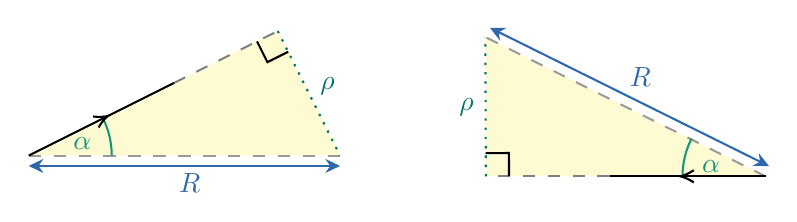
\begin{tikzpicture}[x=0.75pt,y=0.75pt,yscale=-1,xscale=1]
		%uncomment if require: \path (0,220); %set diagram left start at 0, and has height of 220
		
		%Straight Lines [id:da7259190554486932] 
		\draw [draw opacity=0][fill={rgb, 255:red, 248; green, 231; blue, 28 }  ,fill opacity=0.2 ]   (40,70) -- (160,10) -- (190,70) -- (40,70) ;
		%Straight Lines [id:da9779749874503482] 
		\draw [color={rgb, 255:red, 128; green, 128; blue, 128 }  ,draw opacity=1 ] [dash pattern={on 4.5pt off 4.5pt}]  (110,35) -- (160,10) ;
		%Straight Lines [id:da8257478216843763] 
		\draw [color={rgb, 255:red, 155; green, 155; blue, 155 }  ,draw opacity=1 ] [dash pattern={on 4.5pt off 4.5pt}]  (40,70) -- (190,70) ;
		%Shape: Arc [id:dp8525286115409573] 
		\draw  [draw opacity=0] (75.65,51.84) .. controls (78.43,57.29) and (80,63.46) .. (80,70) -- (40,70) -- cycle ; \draw  [color={rgb, 255:red, 17; green, 151; blue, 122 }  ,draw opacity=1 ] (75.65,51.84) .. controls (78.43,57.29) and (80,63.46) .. (80,70) ;  
		%Straight Lines [id:da9176470612228212] 
		\draw [color={rgb, 255:red, 46; green, 104; blue, 172 }  ,draw opacity=1 ]   (43,75) -- (187,75) ;
		\draw [shift={(190,75)}, rotate = 180] [fill={rgb, 255:red, 46; green, 104; blue, 172 }  ,fill opacity=1 ][line width=0.08]  [draw opacity=0] (7.14,-3.43) -- (0,0) -- (7.14,3.43) -- (4.74,0) -- cycle    ;
		\draw [shift={(40,75)}, rotate = 0] [fill={rgb, 255:red, 46; green, 104; blue, 172 }  ,fill opacity=1 ][line width=0.08]  [draw opacity=0] (7.14,-3.43) -- (0,0) -- (7.14,3.43) -- (4.74,0) -- cycle    ;
		%Straight Lines [id:da2817599186584464] 
		\draw [color={rgb, 255:red, 0; green, 116; blue, 102 }  ,draw opacity=1 ] [dash pattern={on 0.84pt off 2.51pt}]  (160,10) -- (190,70) ;
		%Straight Lines [id:da8916062585500438] 
		\draw    (40,70) -- (110,35) ;
		\draw [shift={(78.22,50.89)}, rotate = 153.43] [color={rgb, 255:red, 0; green, 0; blue, 0 }  ][line width=0.75]    (6.56,-2.94) .. controls (4.17,-1.38) and (1.99,-0.4) .. (0,0) .. controls (1.99,0.4) and (4.17,1.38) .. (6.56,2.94)   ;
		%Straight Lines [id:da11392872153871136] 
		\draw    (150,15) -- (155,25) -- (165,20) ;
		%Straight Lines [id:da6493310814500558] 
		\draw [draw opacity=0][fill={rgb, 255:red, 248; green, 231; blue, 28 }  ,fill opacity=0.2 ]   (260.23,80) -- (260,12.92) -- (395,80) ;
		%Straight Lines [id:da5442441210170875] 
		\draw [color={rgb, 255:red, 128; green, 128; blue, 128 }  ,draw opacity=1 ] [dash pattern={on 4.5pt off 4.5pt}]  (320,80) -- (260,80) ;
		%Straight Lines [id:da7510858484660925] 
		\draw [color={rgb, 255:red, 155; green, 155; blue, 155 }  ,draw opacity=1 ] [dash pattern={on 4.5pt off 4.5pt}]  (395,80) -- (260,12.92) ;
		%Shape: Arc [id:dp6145976977724383] 
		\draw  [draw opacity=0] (359.35,61.84) .. controls (356.57,67.29) and (355,73.46) .. (355,80) -- (395,80) -- cycle ; \draw  [color={rgb, 255:red, 17; green, 151; blue, 122 }  ,draw opacity=1 ] (359.35,61.84) .. controls (356.57,67.29) and (355,73.46) .. (355,80) ;  
		%Straight Lines [id:da11786511909673236] 
		\draw [color={rgb, 255:red, 46; green, 104; blue, 172 }  ,draw opacity=1 ]   (393.92,73.73) -- (264.91,9.77) ;
		\draw [shift={(262.22,8.44)}, rotate = 26.37] [fill={rgb, 255:red, 46; green, 104; blue, 172 }  ,fill opacity=1 ][line width=0.08]  [draw opacity=0] (7.14,-3.43) -- (0,0) -- (7.14,3.43) -- (4.74,0) -- cycle    ;
		\draw [shift={(396.61,75.06)}, rotate = 206.37] [fill={rgb, 255:red, 46; green, 104; blue, 172 }  ,fill opacity=1 ][line width=0.08]  [draw opacity=0] (7.14,-3.43) -- (0,0) -- (7.14,3.43) -- (4.74,0) -- cycle    ;
		%Straight Lines [id:da3437761820088857] 
		\draw [color={rgb, 255:red, 0; green, 116; blue, 102 }  ,draw opacity=1 ] [dash pattern={on 0.84pt off 2.51pt}]  (260.23,80) -- (260,12.92) ;
		%Straight Lines [id:da7501678951641484] 
		\draw    (395,80) -- (320,80) ;
		\draw [shift={(353.9,80)}, rotate = 360] [color={rgb, 255:red, 0; green, 0; blue, 0 }  ][line width=0.75]    (6.56,-2.94) .. controls (4.17,-1.38) and (1.99,-0.4) .. (0,0) .. controls (1.99,0.4) and (4.17,1.38) .. (6.56,2.94)   ;
		%Straight Lines [id:da2730983383726572] 
		\draw    (271.41,79.96) -- (271.37,68.78) -- (268.46,68.79) -- (260.19,68.82) ;
		
		% Text Node
		\draw (111,77) node [anchor=north west][inner sep=0.75pt]  [color={rgb, 255:red, 46; green, 104; blue, 172 }  ,opacity=1 ] [align=left] {$\displaystyle R$};
		% Text Node
		\draw (60,60) node [anchor=north west][inner sep=0.75pt]  [color={rgb, 255:red, 17; green, 151; blue, 122 }  ,opacity=1 ] [align=left] {$\displaystyle \alpha $};
		% Text Node
		\draw (179,31) node [anchor=north west][inner sep=0.75pt]  [color={rgb, 255:red, 0; green, 116; blue, 102 }  ,opacity=1 ] [align=left] {$\displaystyle \rho $};
		% Text Node
		\draw (328,26) node [anchor=north west][inner sep=0.75pt]  [color={rgb, 255:red, 46; green, 104; blue, 172 }  ,opacity=1 ] [align=left] {$\displaystyle R$};
		% Text Node
		\draw (363,71) node [anchor=north west][inner sep=0.75pt]  [color={rgb, 255:red, 17; green, 151; blue, 122 }  ,opacity=1 ] [align=left] {$\displaystyle \alpha $};
		% Text Node
		\draw (246,41) node [anchor=north west][inner sep=0.75pt]  [color={rgb, 255:red, 0; green, 116; blue, 102 }  ,opacity=1 ] [align=left] {$\displaystyle \rho $};
	\end{tikzpicture}
\end{figure}

Tenemos que
\begin{equation}
	\sin\alpha = \frac{\rho}{R_{1}}, ~~~~~ \sin\beta = \frac{\rho}{R_{2}}
\end{equation}
Por lo que
\begin{equation*}
	\theta = \arcsin\frac{\rho}{R_{1}} + \arcsin\frac{\rho}{R_{2}}
\end{equation*}
pero \(R_{1} = R_{2} = R\)
\begin{equation}
	\theta = 2 \arcsin\frac{\rho}{R} \label{theta}
\end{equation}
\begin{equation}
	\alpha = \beta
\end{equation}

% % % % % % % % % % % % % % % % % % % % % % % % % % % % % % % % % % % % % % % % % % % % % % % % % % % % % %

\begin{enumerate}
	\item[\textbf{b.}] Find the potential \(U(r)\) which satisfies these properties.
\end{enumerate}

Adaptaremos la ecuación de \(\theta(\rho)\) a
\begin{equation}
	\theta(\alpha) = 2 \Theta(R(1-\alpha))\arcsin\alpha
\end{equation}
donde \(\alpha = \rho / R\). Ahora, aplicando
\begin{equation}
	w(r) \equiv \sqrt{1 - \frac{U(r)}{E} } = \exp\left( \frac{1}{\pi } \int_{r w}^{\infty} \frac{\theta (\rho)}{\sqrt{\rho^2 - r^2 w^2} } \, d\rho \right) \label{w}
\end{equation}
con el cambio de variables la integral:
\begin{equation}
	\int_{\frac{r w}{R}}^1 \frac{\theta (R \,\alpha)}{\sqrt{\alpha ^2 R^2-r^2 w^2}} \, R \, d\alpha = \left\lbrace \begin{matrix}
		-\ln\left[\frac{R}{\sqrt{R^2-r^2 w^2}+R}\right], & r < R\\
		\hfill 0 \hfill, & r > R
	\end{matrix}\right.
\end{equation}
y entonces, considerando el caso \(r < R\)
\begin{align}
	w(r) &= \exp \left(-\ln\left[\frac{R}{\sqrt{R^2-r^2 w^2}+R}\right]\right)\nonumber\\
	&= \frac{\sqrt{R^2-r^2 w^2}+R}{R}\nonumber\\
	\Rightarrow w(r < R) &= \frac{2 R^2}{R^2 + r^2}
\end{align}
mientras que en el caso \(r > R\)
\begin{equation}
	w(r > R) = 1
\end{equation}
Finalmente, resolviendo la ec. \ref{w} para \(U(r)\) tendremos
\begin{equation}
	U(r) = \left\lbrace \begin{matrix}
		E \dfrac{\left(r^4+2 r^2 R^2-3 R^4\right)}{\left(r^2+R^2\right)^2}, & r < R \vspace{3mm}\\
		\hfill 0 \hfill, & r > R
	\end{matrix}\right.
\end{equation}

% % % % % % % % % % % % % % % % % % % % % % % % % % % % % % % % % % % % % % % % % % % % % % % % % % % % % %

\begin{enumerate}
	\item[\textbf{c.}] Assume that we analyze scattering of a collinear beam of monochromatic particles in the field which You found earlier. Find the cross-section of elastic scattering \(d\sigma/d\Omega\) for this case.
\end{enumerate}
Sabemos que
\begin{equation}
	\td{\sigma}{\Omega} = \frac{\rho}{\sin\theta}\left|\td{\rho}{\theta}\right|
\end{equation}
Y, a partir de la ec. \ref{theta}
\begin{equation}
	\rho(\theta) = R \sin\frac{\theta}{2}
\end{equation}
Por lo que, reemplazando y resolviendo
\begin{align}
	\td{\sigma}{\Omega} &= \frac{\rho}{\sin\theta}\left|\td{\rho}{\theta}\right|\nonumber\\
	&= R \frac{\sin\theta/2}{\sin\theta} \left|\frac{1}{2} R \cos\theta/2\right| \nonumber\\
	&= \left\lbrace \begin{matrix}
		\hfill{R^2}/{4},	& \theta < \pi \vspace{3mm}\\
		-{R^2}/{4}, 		& \theta > \pi
	\end{matrix}\right.
\end{align}

\end{document}